\documentclass{article}
\usepackage{graphicx}
\usepackage[utf8]{inputenc}
\usepackage{fullpage}
\usepackage{xcolor}
\usepackage{url}

\parindent0in
\pagestyle{plain}
\thispagestyle{plain}

\newcommand{\myname}{John Doe}
\newcommand{\assignment}{Laboratorio 1}
\newcommand{\duedate}{27 de Mayo, 2018}

\renewcommand\thesubsection{\arabic{subsection}}

\title{Análisis de Algoritmos de Ordenación}
\date{}

\begin{document}

Universidad Católica San Pablo\hfill\\
Algoritmos y Estructura de Datos\hfill\textbf{\assignment}\\
Prof.\ Jorge Poco\hfill\textbf{Entrega:}: \duedate\\
Alumno: Moreno Vera Felipe Adrian
\smallskip\hrule\bigskip

{\let\newpage\relax\maketitle}
\maketitle


Implementar el \emph{insert sort}, \emph{merge sort} y \emph{quick sort} usando el template que se esta anexando (main.cpp) y realizar los siguientes experimentos. En caso tengan problemas con los RandomAccessIterator, les recomiendo ver el siguiente link \url{https://goo.gl/v9QWs3}.

\begin{itemize}
  \item Crear 10 conjuntos de números en orden aleatorio. Los conjuntos deben tener {100 mil, 200 mil, ... 1 millón}. 
  \item Ordenar estos números usando los 3 algoritmos y calcular el tiempo que demora cada algoritmo para cada conjunto de números
  \item Generar una gráfica (usando excel u otra herramienta) mostrando un \emph{linechart}, donde el eje X es el “número de elementos”, y el  eje Y sea el tiempo que demoró el algoritmo. Esta gráfica tiene que tener 3 líneas de diferentes colores con su leyenda. 
  \item Agregar un pequeño párrafo describiendo los resultados.
\end{itemize}

\section{Orden Aleatorio}
Ordenar datos de entrada en orden aleatorio.\\
Debido a la diferencia de tiempos abismales entre el Insertion y Merge-Quick, no es posible realizar una gráfica que abarque a los 3, por lo cual se presenta a través de la Tabla 1.\\

\begin{center}
\begin{tabular}{|l|l|l|l|}
\hline
numdatos & insertion & merge & quick\\
\hline
100000 & 134.493 & 0.24916 & 0.056112\\
200000 & 548.301 & 0.469198 & 0.128171\\
300000 & 1230.29 & 0.706214 & 0.169476\\
400000 & 1903.11 & 0.984869 & 0.193734\\
500000 & 2869.2 & 1.10952 & 0.268326\\
600000 & 3934.62 & 1.25432 & 0.283447\\
700000 & 5262.8 & 1.4952 & 0.381047\\
800000 & 6870.43 & 1.65556 & 0.367589\\
900000 & 8679.01 & 1.92917 & 0.499127\\
1000000 & 10726 & 2.06818 & 0.473238\\
\hline
\end{tabular}\\

Tabla 1 Tabla de Tiempos de ordenamiento de los datos en orden aleatorio.
\end{center}

Se aprecia también que con Insertion Sort, al ser $O(n^2)$, su orden de crecimiento es exponencial a comparación de MergeSort y QuickSort que son O(nlog(n)).

\newpage

\section{Orden Ascendente}
Ordenar datos de entrada en orden ascendente
Se puede apreciar que cuando estan en orden ascendente, InsertionSort mejora considerablemente su tiempo, siendo incluso mucho más rápido que quicksort y mergesort, QuickSort y MergeSort también mejoran su tiempo de ordenamiento pero a un nivel ínfimo.\\

Como se aprecia en la Tabla 2, se puede ver la mejora del InsertionSort, tiempos que si podemos representar en la Figura 1 a diferencia del anterior.\\

\begin{center}
\begin{tabular}{|l|l|l|l|}
\hline
numdatos & insertion & merge & quick\\
\hline
100000 & 0.004997 & 0.170837 & 0.026876\\
200000 & 0.004933 & 0.343593 & 0.055895\\
300000 & 0.007346 & 0.533465 & 0.087575\\
400000 & 0.009812 & 0.722545 & 0.117785\\
500000 & 0.012284 & 0.913763 & 0.149424\\
600000 & 0.015226 & 1.10988 & 0.181855\\
700000 & 0.017343 & 1.30833 & 0.215424\\
800000 & 0.019642 & 1.51211 & 0.245767\\
900000 & 0.02224 & 1.70902 & 0.280971\\
1000000 & 0.024732 & 1.91053 & 0.311758\\
\hline
\end{tabular}\\

Tabla 2 Tabla de Tiempos de ordenamiento de los datos en orden ascendente.
\end{center}

\begin{center}
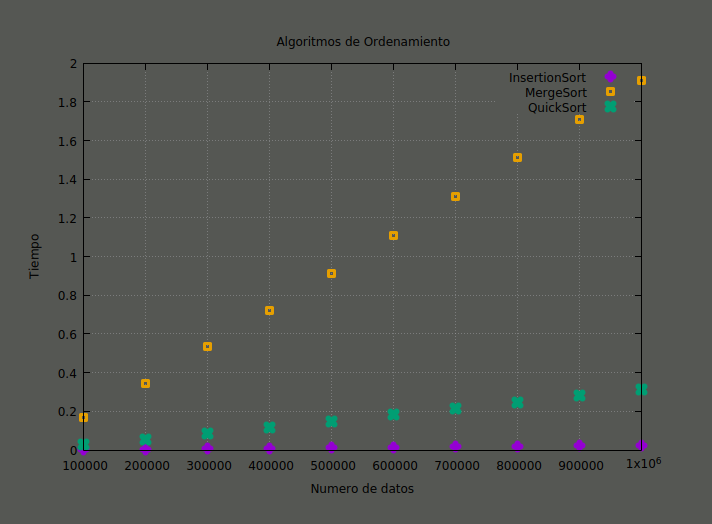
\includegraphics[width=9cm]{grafico_ascendente.png}\\

Fig.1 Gráfica de tiempos de los datos en orden ascendente.
\end{center}

\section{Orden Descendente}
Ordenar datos de entrada en orden descendente.

Se aprecia que los tiempos de ordenamiento, en los 3 casos aumenta, siendo el más extenso el InsertionSort que demoro acerca de 80284 segundos (22:20 horas), tal como se muestra en la Tabla 3.\\

De lo cual se ve que para mayor cantidad de datos en orden descendente, el tiempo de ordenamiento incrementa a diferencia que cuando esta en orden aleatorio (debido a que encuentra tramos ya ordenados, haciendolos un ordenamiento estable).

\begin{center}
\begin{tabular}{|l|l|l|l|}
\hline
numdatos & insertion & merge & quick\\
\hline
100000 & 238.626 & 0.183528 & 0.028501\\
200000 & 914.334 & 0.378737 & 0.05778\\
300000 & 2041.02 & 0.544844 & 0.08908\\
400000 & 3634.66 & 0.739224 & 0.126681\\
500000 & 5618.31 & 0.925705 & 0.153747\\
600000 & 8727.88 & 1.4703 & 0.233881\\
700000 & 11933.9 & 1.33953 & 0.210096\\
800000 & 13394.3 & 1.52303 & 0.241718\\
900000 & 17185.5 & 1.88907 & 0.331368\\
1000000 & 80284.2 & 7.38704 & 1.21763\\
\hline
\end{tabular}\\

Tabla 3 Tabla de Tiempos de ordenamiento de los datos en orden descendente.
\end{center}


\end{document}